%#######################################
% Original: Oktober.2011; Prof. Dr. Martin Grüttmüller, FIM
% Last Edit: Dezember.2021; M.Eng. Mario Hoffmann, Fakultät DIT
% Reimport: April.2022; Prof. Dr. Jean-Alexander Müller, Fakultät Informatik und Medien
%#######################################

%!TEX TS-program = lualatex
%!TEX encoding = UTF-8 Unicode
%!TEX root = MusterAbschlussarbeit.tex
%!TEX spellcheck = de_DE
%!BIB program = biber

\documentclass[a4paper,12pt,numbers=noenddot,parskip,toc=flat,toc=listof,toc=bibliography,twoside=false,captions=tableheading]{scrbook}

%##########################################################
% Dokumentenangaben
%##########################################################
%########## INB
%\newcommand{\abschlussarbeit}{Bachelorarbeit}
%\newcommand{\studiengang}{Informatik}
%\newcommand{\studienganggrad}{Bachelor of Science}
%########## INM
\newcommand{\abschlussarbeit}{Masterarbeit}
\newcommand{\studiengang}{Informatik}
\newcommand{\studienganggrad}{Master of Science}
%########## EoStudiengang
\newcommand{\autor}{VORNAME NACHNAME}
\newcommand{\geburtsort}{GEBURTSORT}
\newcommand{\geburtstag}{GEBURTSTAG}
\newcommand{\titel}{TITEL}
% Falls kein Untertitel, einfach leer lassen
\newcommand{\subtitel}{UNTERTITEL}
\newcommand{\fakultät}{Informatik und Medien}
\newcommand{\erstgutachter}{NAME ERSTGUTACHTER}
\newcommand{\instituteErstgutachter}{INSTITUT}
\newcommand{\zweitgutachter}{NAME ZWEITGUTACHTER}
\newcommand{\instituteZweitgutachter}{INSTITUT}
\newcommand{\ort}{ORT}

% Im Fall eines Themas seitens eines Praxispartners --> Sperrvermerke sind genehmigungs-
% pflichtig!
\newcommand{\betrieb}{BETRIEB}

%##########################################################
% Einbinden aller Pakete etc.
%##########################################################

%!TeX root = ./../MusterAbschlussarbeit.tex


%##########################################################
% Pakete - Stil, Sprache und Schriftart
%##########################################################
\usepackage[UKenglish,ngerman]{babel}
\usepackage[T1]{fontenc}
\usepackage[osf,scale=1.15]{sourcesanspro}
\usepackage{csquotes}
\usepackage[backend=biber,sorting=none,bibencoding=utf8]{biblatex}
\addbibresource{MusterBachelorArbeitBib.bib}
\usepackage[headsepline]{scrlayer-scrpage}
\usepackage{fontspec}
\setcounter{tocdepth}{\subsubsectiontocdepth}
\addtokomafont{chapterentry}{\bfseries}
\usepackage[onehalfspacing]{setspace}
%## #### #### ####### ###
\usepackage[absolute, overlay]{textpos}
\usepackage{svg}
%\DeclareGraphicsExtensions{.png,.jpg,.gif,.pdf,.svg}
%\renewcommand\includesvg[2][]{\includegraphics{#2}}

\AtBeginDocument{%
	\providecaptionname{ngerman}{\lstlistlistingname}{Quellcodeverzeichnis}
	\providecaptionname{ngerman}{\lstlistingname}{Quellcode}
}

%##########################################################
% Pakete - Grafisches Elemente und Farben
%##########################################################
\usepackage{graphicx}
\usepackage{xcolor}

\providecommand{\keywords}[1]{\textbf{\textit{Keywords:}} #1}

%############ HTWK Farben #################
\xdefinecolor{htwkGelb}{rgb}{0.996,0.925,0}
\xdefinecolor{htwkGrau}{rgb}{0.945,0.945,0.945}
\xdefinecolor{htwkBlau}{rgb}{0,0.273,0.597}
\xdefinecolor{htwkMagenta}{rgb}{0.894,0,0.488}
\xdefinecolor{htwkRot}{rgb}{0.894,0.1875,0.035}
\xdefinecolor{htwkGruen}{rgb}{0,0.586,0.304}
\xdefinecolor{htwkCyan}{rgb}{0,0.617,0.886}
\xdefinecolor{codegreen}{rgb}{0,0.6,0}
%######## Legen Sie die Farbe fest #####
% htwkBlau, htwkGruen, htwkRot, htwkCyan, htwkGelb, htwkMagenta, htwkGrau
\newcommand{\farbe}{htwkBlau}
%#########################################

%Linkformatierung
\usepackage[
	    colorlinks=true,
	    urlcolor=htwkBlau,
	    citecolor=htwkBlau,
		pdftitle={\titel},
		pdfauthor={\autor},
		breaklinks=true,
		hidelinks
]{hyperref}

%##########################################################
% Pakete - Zusätzliche
%##########################################################

\usepackage{listings}
\usepackage{scrhack}
\usepackage{microtype}
\usepackage{acro}

%##########################################################
% Code Snippet Definitionen
%##########################################################
\newcommand\digitstyle{\color{purple}}
\makeatletter
\newcommand{\ProcessDigit}[1]
{%
  \ifnum\lst@mode=\lst@Pmode\relax%
   {\digitstyle #1}%
  \else
    #1%
  \fi
}

\lstdefinestyle{MyStyle}{
	basicstyle=\footnotesize\sffamily,
	keywordstyle=\color{blue},
	commentstyle=\color{codegreen},
	stringstyle=\color{orange!80!black},
	morecomment=[l]{//},
	morecomment=[l]{/*}{*/},
	morestring=[b]",
	morestring=[b]',
	breakatwhitespace=false,         
    breaklines=true,                 
    keepspaces=true,
	showspaces=false,                
    showstringspaces=false,
    showtabs=false,                  
    tabsize=2,
	numbers=left,
	numberstyle=\tiny,
	frameround=tttt,
	frame=trbl,
	columns=fullflexible,
	xleftmargin=0.03\linewidth,
	xrightmargin=0.01\linewidth,
	inputencoding=utf8,
}

\lstset{
	style=MyStyle,
	literate=%
    {0}{{{\ProcessDigit{0}}}}1
    {1}{{{\ProcessDigit{1}}}}1
    {2}{{{\ProcessDigit{2}}}}1
    {3}{{{\ProcessDigit{3}}}}1
    {4}{{{\ProcessDigit{4}}}}1
    {5}{{{\ProcessDigit{5}}}}1
    {6}{{{\ProcessDigit{6}}}}1
    {7}{{{\ProcessDigit{7}}}}1
    {8}{{{\ProcessDigit{8}}}}1
    {9}{{{\ProcessDigit{9}}}}1
}

%!TeX root = ./../MusterAbschlussarbeit.tex

%##########################################################
% Inhalt
%##########################################################

\DeclareAcronym{htwk}{
    short = HTWK,
    long = Hochschule für Technik{,} Wirtschaft und Kultur Leipzig
}

\DeclareAcronym{fim}{
    short = FIM,
    long = Fakultät Informatik und Medien
}

\DeclareAcronym{ppo}{
    short = PPO,
    long = Proximal Policy Optimization
}

\DeclareAcronym{sac}{
    short = SAC,
    long = Soft Actor Critic
}

\DeclareAcronym{ml}{
    short = ML,
    long = Machine Learning
}


\DeclareAcronym{rl}{
    short = RL,
    long = Reinforcement Learning
}

\DeclareAcronym{ftth}{
    short = FTTH,
    long = Fiber to the Home
}

\DeclareAcronym{html}{
    short = HTML,
    long = Hypertext Markup Language
}


%##########################################################
% Begin des Dokumentes
%##########################################################
\begin{document}

%!TeX root = ./../MusterAbschlussarbeit.tex

\pagestyle{scrheadings}
\clearpairofpagestyles

\ofoot[\pagemark]{\pagemark}
\ohead{\headmark}
\automark{chapter}

%!TeX root = ./../MusterAbschlussarbeit.tex

%##########################################################
% Titelseite
%##########################################################

\begin{titlepage}
	\noindent
\begin{textblock*}{4.74cm}(16.7mm,11mm)
\includegraphics[width=4.74cm]{Bilder/logos/HTWK-Fakultaetszusatz_IM_schwarz_de-eps-converted-to.pdf}
\end{textblock*}
\begin{center}

\vspace*{0.5cm}

\large
{\textsc{\Large \abschlussarbeit}}

\vspace*{0.5cm}
zur Erlangung des akademischen Grades\\[0.6cm]
\studienganggrad\\[0.6cm]
im Studiengang \studiengang\\
der Fakultät \fakultät\\
der Hochschule für Technik, Wirtschaft und Kultur Leipzig

{\LARGE \textbf{\titel}}\\
{\LARGE \textbf{-- \subtitel --}}

\end{center}

%##########################################################
% Autor/in
%##########################################################

\vspace*{2cm}
vorgelegt von: \autor \\
Geburtsort und -datum: \geburtsort, den \geburtstag \\
Abgabe: \ort, den \today



\vspace*{1cm}
\large
\begin{tabbing}
\hspace{4cm}\=\kill
Erstgutachter:  \> \erstgutachter, \\ \> \instituteErstgutachter\\ 
Zweitgutachter:  \> \zweitgutachter, \\ \> \instituteZweitgutachter
\end{tabbing} 

\begin{textblock*}{8.41cm}(18mm,268.3mm)
\includegraphics[width=8.41cm]{Bilder/logos/htwk-logo-eps-converted-to.pdf}
\end{textblock*}

\end{titlepage}


%##########################################################
% Sperrvermerk
% Ist vorher abzuklären!
%##########################################################
\pagenumbering{gobble}
%%!TeX root = ./../MusterAbschlussarbeit.tex

%##########################################################
% Inhalt
%##########################################################

\thispagestyle{empty} % no page number
\chapter*{Sperrvermerk}

\noindent
Die vorliegende Bachelorarbeit mit dem Titel \titel{} beinhaltet interne vertrauliche Informationen der Firma \betrieb{} des Autors oder patentrechtlich relevante Informationen. 

Die Weitergabe des gesperrten Inhaltes der Arbeit und eventuell beiliegender
Zeichnungen und Daten im Gesamten oder in Teilen ist grundsätzlich untersagt. Es dürfen keinerlei Kopien oder
Abschriften -- auch in digitaler Form -- gefertigt werden. 
Ausnahmen bedürfen der vorherigen schriftlichen Genehmigung der Firma \betrieb{} oder des Autors.

%Hier kommen die Unterschriften hin
\vspace{1.5cm}
\begin{tabular}{p{7cm}p{.5cm}p{7cm}}
	\dotfill & & \dotfill \\\\
	Ort, Datum, Unterschrift \erstgutachter & & Ort, Datum, Unterschrift \zweitgutachter \\
    & & \\\\
    & & \\\\
    \dotfill \\\\
    Ort, Datum, Unterschrift \autor
\end{tabular}


%##########################################################
% Eidesstaatliche Erklärung
%##########################################################
%!TeX root = ./../MusterAbschlussarbeit.tex

%##########################################################
% Inhalt
%##########################################################

\clearpage
\thispagestyle{empty}
\chapter*{Eidesstattliche Erklärung}

Hiermit erkläre ich, dass ich die an der Hochschule für Technik, Wirtschaft und Kultur Leipzig, konkret an der \ac{fim}, eingereichte Arbeit zum Thema \titel{} selbstständig, ohne Hilfe Dritter und ohne Benutzung anderer als der angegebenen Quellen und Hilfsmittel verfasst habe. 

Alle den benutzten Quellen wörtlich oder sinngemäß entnommenen Stellen sind als solche einzeln kenntlich gemacht. Die Abbildungen in dieser Arbeit wurden von mir selbst erstellt oder mit einem entsprechenden Hinweis auf die Quelle versehen.

Diese Arbeit ist bislang keiner anderen Prüfungsbehörde vorgelegt und auch nicht veröffentlicht worden.

Ich bin mir bewusst, dass eine falsche Erklärung rechtliche Folgen haben wird.

\noindent

\vspace{3cm}
\begin{tabular}{p{7cm}p{.5cm}}
    \dotfill \\\\
    Unterschrift \autor\\
    \ort, den \today
\end{tabular}



%##########################################################
% Vorwort (optional)
%##########################################################
%!TeX root = ./../MusterAbschlussarbeit.tex

%##########################################################
% Inhalt
%##########################################################
\clearpage
\chapter*{Vorwort (optional)}
In einem Vorwort können persönliche Danksagungen, Ihre eigene Motivation sowie persönliche Erkenntnisse niederschreiben. 
Inhaltliche Angaben zum Werk werden jedoch nicht gemacht. Zudem ist es möglich hier eine Gendererklärung abzugeben.
Gendererklärung:
In dieser Arbeit wird aus Gründen der besseren Lesbarkeit das generische Maskulinum verwendet. 
Weibliche und anderweitige Geschlechteridentitäten werden dabei ausdrücklich mitgemeint, soweit es für die Aussage erforderlich ist.


%##########################################################
% Abstract/Kurzfassung
%##########################################################
%!TeX root = ./../MusterAbschlussarbeit.tex

%##########################################################
% Inhalt
%##########################################################

\clearpage
\chapter*{Kurzfassung}
Die Kurzfassung - präziser: Abstrakt, sollte auf eine Seite beschränkt sein. Der Abstrakt
sollte das Ziel der Arbeit explizit beschreiben, die angewandten \textit{Methoden} aufführen, die
wichtigsten \textit{Ergebnisse} aufzählen und die \textit{Hauptschlussfolgerungen} aufzeigen.

Einen Weg zu finden, hunderte von Seiten an Informationen in wenigen Sätzen zusammenzufassen
ist eine Herausforderung. Jedes Wort muss sorgfältig abgewogen werden
(Gibt es eine bessere, prägnantere Möglichkeit, die Hauptaussage auszudrücken?). Die
einzelnen Sätze sollten mit größter sorgfalt kombiniert werden.

Das Verfassen des Abstraktes sollte bis zum Schluss aufgeschoben werden, aus dem
selben Grund, warum der Titel der Arbeit erst dann endgültige Form erhalten sollte,
wenn das entsprechende Arbeit ansonsten vollständig ist.

Die nachfolgenden Ausführungen sollen nochmal ins Gedächtnis rufen was die Anforderungen an einzelne Abschnitte einer Abschlussarbeit
an der \ac{fim} der \ac{htwk} sind.

Die Kurzfassung schließt mit der Nennung von 5 bis 10 Schlagwörtern (Keywords) ab,
welche der Verschlagwortung bspw. für die Recherche nutzbar gemacht werden. Genauer gesagt, sind das inhaltliche Schlüsselwörter Ihrer Arbeit.\\\\



Die Struktur dieser Arbeit gliedert sich wie folgt:
\setlist{noitemsep}
\begin{itemize}

    \item \textbf{Theoretische Grundlagen:} In diesem Abschnitt werden die grundlegenden Konzepte des Reinforcement Learning erläutert, darunter Neuronale Netze Markov-Entscheidungsprozesse und Probleme welche beim dem RL auftreten können. Weiterhin wird eine detaillierte Beschreibung des Spiels 'Noch mal' gegeben, einschließlich der Regeln, Spielziele und möglicher Strategien.
    \item \textbf{Konzeption:} Dieser Abschnitt umfasst eine Anforderungsanalyse und  beschreibt den Ansatz zur Implementierung des Reinforcement Learning-Agenten für 'Noch mal'. 
    \item \textbf{Experimente und Ergebnisse:} Es werden die Ergebnisse der Experimente präsentiert, einschließlich der Leistung des RL-Agenten beim Spielen von 'Noch mal' und einer Analyse seiner Fähigkeiten und Schwächen.
    \item \textbf{Diskussion:} Eine Diskussion über die Ergebnisse, die Einschränkungen der Studie und mögliche Verbesserungen wird vorgenommen.
    \item \textbf{Fazit und Ausblick:} Abschließend werden die wichtigsten Erkenntnisse zusammengefasst und ein Ausblick auf mögliche zukünftige Forschungsrichtungen gegeben.
\end{itemize}


\keywords{IoT, SD-WAN, \ac{ml}, \ac{ftth}}


%##########################################################
% Inhaltsverzeichnis
%##########################################################
\tableofcontents

%##########################################################
% Abbildungsverzeichnis
%##########################################################
\listoffigures

%##########################################################
% Tabellenverzeichnis
%##########################################################\
\listoftables

%##########################################################
% Quelltextverzeichnis
%##########################################################\
\lstlistoflistings
\clearpage

%##########################################################
% Abkürzungsverzeichnis
%##########################################################
\printacronyms[name=Abkürzungsverzeichnis, heading=chapter*]
\addcontentsline{toc}{chapter}{Abkürzungsverzeichnis}

%##########################################################
% Erstes Kapitel
%##########################################################
%!TeX root = ./../MusterAbschlussarbeit.tex

%##########################################################
% Inhalt
%##########################################################
\pagenumbering{arabic}
\chapter{Einleitung}

Der Leser Ihrer Arbeit sollte die Einleitung (auch als \enquote{Hintergrund} oder \enquote{Problemstellung} bezeichnet) als eine Art Rundblick erleben, 
der die Landschaft darstellt, mit der der Autor konfrontiert wurde, als die Arbeit entstand. Wann und wie hat sich dieses Forschungsthema erstmals angeboten? 
Was hat deutlich gemacht, dass es interessante Fragen gibt, die beantwortet werden müssen? Welche Handlungen und Zusammenhänge waren damals schon erkennbar, und welche Schlüsselinformationen fehlten? 

In der Regel wird in der Einleitung auch ein methodischer Ansatz zur Lösung des Problems vorgeschlagen, 
der möglicherweise durch konkrete Beispiele für die Anwendung dieses Ansatzes unter anderen Umständen veranschaulicht wird. 
Achten Sie beim Schreiben darauf, dass Sie klar zwischen Ihrer Arbeit und anderen Beiträgen unterscheiden müssen.

Bei umfangreichem Material, das Sie hier behandeln möchten, könnte es sich lohnen, die Einleitung in Unterabschnitte zu unterteilen.

Kein anderer Abschnitt in der Arbeit hängt so sehr von der Literaturrecherche ab wie die Einleitung \cite{aoscw2004}. 
Bevor Sie mit der Arbeit an Ihrem Projekt begonnen haben, haben Sie sicher einige wichtige Hintergrundartikel gelesen, 
die Ihnen Ihr Betreuer schon empfohlen hat, aber Sie haben sie wahrscheinlich in letzter Zeit nicht mehr gelesen. 
Jetzt müssen Sie diese nicht nur erneut lesen, sondern sich auch eingehend mit den darin enthaltenen Verweisen befassen, 
um sich mit allen wichtigen Informationsquellen vertraut zu machen. Dies wird Sie natürlich auch in die Lage versetzen, 
frühere Arbeiten kritisch zu bewerten.

\newpage

\section{Ein Beispielabschnitt mit diversen Dingen und Erläuterungen}
Zunächst ein Beispiel für Tabellen. Wichtig ist, dass die Tabellenbeschriftung a) da ist und b) \underline{über} der Tabelle steht. Die Lesenden wollen wissen was sie sehen, bevor sie in die Tabelle eintauchen.
Die hier gezeigte Tabelle ist ohne zusätzliche Pakete verwendbar. Alternativ wäre \texttt{longtable} einzubinden und zu verwenden.

\begin{table}[!h]
    \caption[Tabellenbeschriftung]{Tabellenbeschriftung \cite{Tane2014}}
    \centering
    \begin{tabular}{|c|c|c|}
        \hline
        ID & Kapitel & Seiten \\\hline
        0 & 1 & 5 \\\hline
    \end{tabular}
    \label{tab:Beispieltabelle}
\end{table}

Darüber hinaus drei Beispiele für Programm-Code. Im Ordner \glqq Programmcode\grqq{} sind drei Beispiele für C-, Python- und \ac{html}-Code, welche nachfolgend eingebunden ist.
Es empfiehlt sich ganze Dateien einzubinden, statt den Quellcode hier abzutippen.\\
Der Style ist fest definiert und muss nicht abgeändert werden. In aller Regel werden alle stilistischen Anliegen erfüllt.\\
Wie Sie im \LaTeX{} Quellcode sehen, ist die Caption direkt in den Aufruf reinzuschreiben. Gleiches gilt für ein Label, welches ich hier \ref{lst:C-Code-Beispiel}, hier \ref{lst:Python-Code-Beispiel} und hier \ref{lst:HTML-Code-Beispiel} referenziere.\\
Die Angabe der Sprache dient dem Zweck, dass sprachspezifische Keywords o.ä. geladen und erkannt werden, damit die Farbgebung passt.

\lstinputlisting[caption=C-Code Beispiel,label={lst:C-Code-Beispiel},language=C]{Programmcode/test.c}
\lstinputlisting[caption=Python-Code Beispiel,label={lst:Python-Code-Beispiel},language=Python]{Programmcode/test.py}

\textbf{Es ist dabei auch darauf zu achten, dass Quelltexte wenn möglich natürlich nicht über das Seitenende gehen sollten, wie z.B. beim Python-Code Bsp. Setzen Sie daher auch manuell
Seitenumbrüche.} Quelltexte welche eine Seite übersteigen, sind ohnehin eher als Anhang zu betrachten $\rightarrow$ siehe dazu Beschreibung im Anhang.

\lstinputlisting[caption=HTML-Code Beispiel,label={lst:HTML-Code-Beispiel},language=HTML]{Programmcode/test.html}

Nachfolgend noch ein einfaches Beispiel ein Bild einzubinden. Da es sich um Bild\textit{unterschriften} handelt, gehört diese somit \underline{unter} die Abbildung, anders als bei Tabellen\textit{überschriften}.\\
Im \LaTeX-Quelltext sieht man die Optionen für das Einbinden des Bildes. Neben \texttt{scale} wäre auch \texttt{width} möglich mit dem Parameter \texttt{linewidth} oder \texttt{textwidth}.\\
Achten Sie vor allem auf die Lesbarkeit der auf dem Bild befindlichen Informationen, unter der stetigen Annahme, dass es sich um ein ausgedrucktes Dokument handelt. Dort gibt es keinen Zoom.

Empfehlenswert wäre soweit möglich mit skalierbaren Vektorgrafiken zu arbeiten. Allerdings müssten Sie diese vor dem Aufruf von LaTeX in PDFs wandeln (inkscape IM-logo.svg -o IM-logo.pdf) oder Inkscape installieren und LaTeX mit --shell-escape aufrufen.

\begin{figure}[!t]
    \centering
    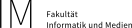
\includegraphics[scale=0.6]{Bilder/logos/IM-logo}
    \caption{Das Logo von Informatik und Medien }
\end{figure}

\begin{figure}[!t]
    \centering
    \includesvg[width=0.6\columnwidth]{Bilder/logos/IM-logo.svg}
    \caption{Das Logo von Informatik und Medien }
\end{figure}

Bedenken Sie bei allen Beschriftungen, egal ob Abbildungen, Tabellen oder Quelltexte, dass Sie, sofern diese nicht Ihrer eigenen Schaffenskraft entsprangen,
diese referenzieren. Im Beispiel der Tabelle \ref{tab:Beispieltabelle} sieht man, dass sich der Beschreibungstext direkt an der Tabelle von dem im Tabellenverzeichnis unterscheidet,
genau um den Punkt der Referenz.

\section{Methodik}

Im Methodik-Abschnitt (eine eigene Section) einer Arbeit stellen Sie die Methoden dar, die Sie verwendet haben oder vorhaben zu verwenden, um die Fragestellung zu beantworten. 
In diesem Abschnitt erläutern Sie, welche Methoden umgesetzt wurden (oder auch angedacht), um die Hypothesen zu testen und die Fallstudie durchzuführen. 
Welche Methoden für Ihre Arbeit geeignet sind, ist auch ein wesentlicher Punkt Ihres angestrebten Titels und somit ein zu bewertender Teil dieser Arbeit. 

\underline{Aber \textbf{mindestens} folgende Punkte}\\
Inhalt des ersten Kapitels (im Allgemeinen):
\begin{itemize}
    \item Thematische Einführung, umreißen des Themas \dots wo befinden wir uns?
    \item Herausstellen des Problems und warum es eines ist was gelöst werden sollte.
    \item Herausstellen der tatsächlichen Ziel-/Fragestellung, welche bearbeitet werden wird.
    \item Eine Abgrenzung was diese Arbeit ist und was sie nicht ist.
    \item Stand der Forschung \dots Was existiert bereits? Wie gut passt das auf das Problem?
    \begin{itemize}
        \item Referenzen mittels cite: \cite[S.~111]{jsch2011} \cite[S.~27f]{Tane2014}
    \end{itemize}
    \item Eine abgeleitete Methodik $\rightarrow$ basierend auf der Literatur und Ihrem Wissen: wie haben Sie nun vor Ihr Problem zu lösen? Vllt durch \cite{9429985}?
\end{itemize}





%##########################################################
% Zweites Kapitel
%##########################################################
%!TeX root = ./../MusterAbschlussarbeit.tex

%##########################################################
% Inhalt
%##########################################################

\clearpage
\chapter{Theoretische Grundlagen}
\section{Neuronale Netze}
Neuronale Netze (=NN) sind ein Modell für künstliche Intelligenz nach dem Vorbild des Gehirns.


Es besteht aus mehreren Schichten verknüpfter Neuronen. Diese verarbeiten numerische Informationen und wandeln diese in einen Output.  In \ref{fig:künstlichesNeuron} ist der Aufbau eines künstlichen Neurons schematisch dargestellt. Jedes Neuron besitzt eine Aktivierungsfunktion, welche entscheidet ob es aktiv ist oder nicht. Neuronen geben Werte von 0 (passiv) bis 1 (aktiv) als Output weiter. 

Um ein NN zu erzeugen, wird eine Vielzahl der Neuronen miteinander verknüpft. Die Ausgänge der vorderen Neuronen sind dabei immer mit den Eingängen der Neuronen der nächsten Schicht verknüpft. \ref{fig:neuronalesNetz} zeigt den Aufbau eines solchen Netzes. 

Wird ein NN initialisiert, werden Kantengewichte zwischen den Neuronen zufällig verteilt. Diese Kantengewichte sorgen dafür wie stark einzelne Neuronen in die nachfolgende Rechnung eingehen.
Deshalb liefern untrainierte NN schlechte Ergebnisse und müssen lernen die Problemstellung richtig zu lösen. Dieser Prozess wird als Training bezeichnet.
Während des Trainings eines NN werden Kantengewichte angepasst, um die Heuristik  an ein optimales Ergebnis anzupassen. Richtig trainierte NN können gute Antworten für komplexe Problemstellungen geben, so liefern sie beispielsweise in der Mustererkennung gute Ergebnisse.\cite{lorenz_reinforcement_2020}
Für das Training von NN wird viel Rechenleistung gebraucht, da der Prozess mit vielen Rechenoperationen verbunden ist.
\cite{ertel_grundkurs_2021}

\begin{figure}[!htb]
	\centering
	\includegraphics[width=0.5\textwidth]{Bilder/künstlichesNeuron.png}
	\caption{Aufbau eines künstlichen Neurons \cite{noauthor_kunstliche_nodate}}
    \label{fig:künstlichesNeuron}
\end{figure}

\begin{figure}[!htb]
	\centering
	\includegraphics[width=0.5\textwidth]{Bilder/AufbauNN.png}
	\caption{Schematische Darstellung eines neuronalen Netzes \cite{noauthor_kunstliche_nodate}}
    \label{fig:neuronalesNetz}
\end{figure}



\clearpage
\section{Reinforcement Learning}
Reinforcement Learning ist ein Bereich des maschinellen Lernens, bei welchem ein Agent durch Interaktion mit seiner Umgebung (Environment) lernt, welche Aktionen in welchen Situationen am besten geeignet sind, um ein bestimmtes Ziel zu erreichen. Da ein Agent keine konkrete Vorgehensweise besitzt, versucht er über Trial-and-Error herrauszufinden welche Aktionen zu Belohnungen führen. \\
Bestandteile des RL sind der Agent und die Umwelt. Der Agent bekommt die Informationen der Umwelt übergeben und entscheidet welche Handlungen daraus folgen sollen. Das Environment setzt die Aktionen des Agenten in Handlungen (Aktionen) um und bewertet diese mit numerischen Belohnungen (Rewards). Anhand der erhaltenen Rewards, versucht der Agent seine Aktionen anzupassen, um die zukünftigen Belohnungen zu maximieren. \\
Ein RL-Agent nimmt seine Umgebung als eine Menge an bestimmten Zuständen wahr.
Jeder Zustand enthält eine Vielzahl von Merkmalen welche für die Entscheidungsfindung relevant sein können.
Als Zustandsraum wird die Menge aller möglichen Zustände bezeichnet.\\
Auf jedem dieser Zustände ist es möglich eine bestimmte Menge an Aktionen auszuführen, welche das Umfeld in einen anderen Zustand überführen.
Die Menge aller möglichen Aktionen wird als Aktionsraum bezeichnet.\\
Wird eine Aktion auf einem bestimmten Zustand ausgeführt, so bezeichnet man die Zustandsübergänge bei Ausführung der Aktion als Zustandsübergangsfunktion.\\
Die Verhaltensstrategie  eines Agenten liefert zu jedem Zustand eine Aktion. Die Policy wird im Verlauf des Trainings erlernt.\\
Das Erlernen einer Policy erfolgt durch Training des Neuronalen Netzes. Zu Beginn des Trainings werden Kantengewichte des zur trainierenden Neuronalen Netzes zufällig verteilt. Um zu überprüfen ob seine Aktionen gut oder schlecht sind, muss der Agent durch einen numerischen Rückgabewert die Information erhalten. Diese numerischen Rückgabewerte werden als Belohnungen (Rewards) bezeichnet. Belohnungen werden vom Zustandsraum verteilt und können gutes Verhalten des Agenten durch positive Rewards und falsches Verhalten durch negative Rewards bestärken.
Der Agent versucht den Wert der erhaltenen Belohnungen zu maximieren und erlernt auf diese Weise eine optimale Policy. \\
\newpage
Probleme, welche beim RL auftreten können, sind unter anderem:  
\begin{itemize}
    \item Überanpassung 
    \item Belohnungsumgehung, 
    \item Sparse Rewards
    \item große Beobachtungsvektoren
\end{itemize}
Von \textbf{Überanpassung} spricht man, wenn der Agent ein Problem gut in der Lernumgebung in welcher er trainiert wurde lösen kann allerdings nicht auf abweichenden Umgebungen. Es tritt auf, wenn der Agent zu spezialisiert auf seine Trainingsumgebung ist und sich nicht an andere Situationen anpassen kann. Diese Problem lässt sich durch Generalisierung des Trainingsprozesses beheben. Ein Agent, welcher in vielen zufällig generierten Umgebungen trainiert, kann deutlich besser mit neuen Situationen umgehen, benötigt im Gegenzug dazu auch mehr Zeit zum Trainieren. \\
\textbf{Belohnungsumgehung} tritt auf, wenn der Agent lernt die Belohnungsfunktion zu manipulieren, um erhaltene Belohnungen zu maximieren, ohne das eigentliche Ziel der Aufgabe zu erreichen. Dies führt zu unerwünschtem Verhalten des Agenten. Verhindert werden kann dieses Problem, indem Belohnungen direkt mit dem Ziel verknüpft werden, also nur Belohnugnen ausgelöst werden, wenn tatsächlich positive Aktionen ausgeführt werden. \\
Von \textbf{Sparse Rewards} spricht man, wenn die Lernumgebung dem Agenten nur selten oder unregelmäßig Belohnungen vergibt. Dies führt dazu, dass der Agent Schwierigkeiten hat, die ihm gegebene Aufgabe richtig zu erlernen. Um dieses Problem zu umgehen, kann man zusätzliche künstliche Belohnungen einführen, welche den Agenten auf den Weg zum richtigen Verhalten führen. Dies kann im Rückschluss jedoch wieder zur Belohnungsumgehung führen, wenn der Agent die Zwischenbelohnungen, nutzt um maximale Belohnungen zu erhalten. \\
Auch ein zu \textbf{großer Beobachtungsvektor} kann zu Komplikationen führen. Wird dem Agenten eine Vielzahl an Observationen zugeführt, müssen erheblich mehr Parameter im Modell verarbeitet werden, was zu größerem Berechnungsaufwand führt. Dadurch wird auch die Lerngeschwindigkeit verlangsamt und der Bedarf an Speicherplatz für die Modelle steigt. So ist es möglich, dass einfach erscheinende Aufgaben mehrere Tage an Rechenzeit benötigen, um ein gutes Modell zu generieren.
\cite{zai_einstieg_2020}

\newpage
\subsection{Markov- Entscheidungsprozess}
Jedes RL Problem lässt sich durch den Markov Entscheidungsprozess (= MDP) beschreiben.
Der MDP ist ein mathematisches Modell für Entscheidungsprobleme, bei welchem der Agent abhängig von der Umwelt Entscheidungen trifft, um ein bestimmtes Ziel zu erreichen.
MDP setzen die Einhaltung der Markov-Eigenschaft vorraus. Diese ist erfüllt, wenn ein Zustandsübergang nur vom letzten Zustand und der letzten Aktion abhängig ist.
Hauptkomponenten des MDP sind eine endliche Menge valider Zustände, eine endliche Menge valider Aktionen, Belohnungsfunktion und Verhaltensstrategie.
Das Ziel eines MDP ist es eine optimale Policy, durch Maximierung der erhaltenen Belohnungen zu ermitteln. \\
\ref{fig:markov} stellt den Ablauf eines MDP dar. Zu Beginn einer Episode, befindet sich die Lernumgebung in einem gewissen Zustand. Dieser Zustand wird dem Agenten übergeben. Anhand der Beobachtungen führt der Agent eine Aktion aus, welche die Umgebung verändert. Die Veränderung der Umgebung erzeugt einen neuen Zustand, welcher im nächsten Schritt wiederum dem Agenten übergeben wird. Durch Auslösen von Aktionen in der Lernumgebung werden Belohnungen erzeugt, welche dem Agenten einen numerischen Wert liefern, ob die Aktion gut oder schlecht war. Der Agent versucht die erhaltenen Belohnungen zu maximieren.
Eine hohe Belohnung impliziert das richtige Verhalten zum Lösen des Problems, welches der Agent bewähltigen muss.
Dieser Prozess wiederholt sich bis das Problem gelöst wurde. \cite{zai_einstieg_2020}

\begin{figure}[!h]
	\centering
	\includegraphics[width=0.7\textwidth]{Bilder/Markov.png}
	\caption{Ablauf eines MDP \cite{zai_einstieg_2020}}
	\label{fig:markov}
\end{figure}

\newpage
\section{Das Würfelspiel: Noch Mal}
Im modellierten Spiel 'Noch Mal!' geht es darum so viele Kästchen wie möglich anzukreuzen und damit viele Spalten und gleichfarbige Kästchen auszufüllen. Jeweils ein Farb- und ein Zahlenwürfel müssen kombiniert werden, um entsprechend verfügbare und zusammenhängende Felder der gewählten Farbe abzukreuzen. Dabei kann der Zahlenwürfel die Werte von eins bis fünf oder einem Joker ergeben. Der Farbwürfel besitzt die fünf Farben des Feldes und einem Joker. Gespielt wird nach folgenden Regeln:
\setlist{noitemsep}
\begin{enumerate}
    \item Felder in der Spalte H sind von Beginn an verfügbar
    \item Alle Kreuze müssen immer zusammenhängend in genau einem Farbblock der gewählten Farbe platziert werden
    \item Kreuze müssen waagerecht oder senkrecht benachbart zu einem bereits abgekreuzten Feld oder Teil der Spalte H sein, um verfügbar zu werden
    \item Es müssen genau so viele Felder angekreuzt werden, wie das Ergebnis des gewählten Zahlenwürfels
    \item Es könnte nicht mehr als 5 Kästchen in einem Zug abgekreuzt werden
    \item Wird ein Zahlenjoker gewählt, darf der Spieler eine Zahl von 1-5 bestimmen
    \item Wird ein Farbjoker gewählt, darf der Spieler eine Farbe bestimmen
\end{enumerate}

Um im Spiel 'Noch mal' eine möglichst hohe Anzahl an Punkten zu erhalten, ist es wichtig nach folgenden Strategien zu spielen:\\
\textbf{Priorisierung äußerer Spalten}: Äußere Spalten geben mehr Punkte, weshalb es wichtig ist diese komplett auszufüllen. \\
\textbf{Beenden von Farben}: Vollständig ausgefüllte Farben geben viele Extrapunkte. Im späten Spielverlauf kann es besser sein Farben komplett zu füllen anstatt Spalten zu werten. \\
 \textbf{Priorisieren von Sternfeldern}: Jedes ausgefüllte Sternfeld gibt 2 Punkte, eine gute Spielweise ist es so viele Sternfelder wie möglich auszufüllen. \\
\textbf{Strategische Nutzung von Jokern}: Ungenutzte Joker geben zum Ende des Spiels Punkte. Es ist gut diese so wenig wie möglich zu nutzen, um Extrapunkte zu bekommen. Jedoch können mit Hilfe von Jokern einfach bestimmte Felder gewählt werden, welche benötigt werden um eine Wertung zu erzielen. 


\begin{figure}[!h]
	\centering
	\includegraphics[width=0.7\textwidth]{Bilder/Abbildung2.png}
	\caption{Vorlage des Spielfedes mit Indikation der Punktewertung 
	\cite{schmidt_spiele_gmbh_spielregeln_nodate}}
	\label{fig:Vorlage}
\end{figure}

Die Grafik \ref{fig:Vorlage} ist ein Spielfeld aus 'Noch mal!'. Nach Vorlage dieses Spielfelds wurde die Lernumgebung für den Agenten modelliert. Die blau markierten Felder geben den Spaltennamen der Spalten an. Die rot markierten Felder zeigen an, wie viele Punkte beim ausfüllen der jeweiligen Spalte erzielt werden. Das grün markierte Feld zeigt die Anzahl der verbleibenden Joker an, wird ein Joker benutzt, muss eines der Felder abgestrichen werden. Zum Ende des Spiels erhält der Spieler Extrapunkte für die verbleibenden Joker. In jeder Spalte befindet sich ein gelb markiertes Sternfeld. Diese geben zum Ende des Spiels Minuspunkte, weshalb es wichtig ist alle Sternfelder auszufüllen. 


\clearpage


\subsection{Spielablauf Einspieler Variante}
Der Spieler hat 30 Züge Zeit, maximale Punkte zu erreichen und würfelt jede Spielrunde alle 4 Würfel, bestehend aus 2 Farb- und 2 Zahlenwürfeln. Anschließend wählt er ein Paar aus Farb- und Zahlenwürfel aus und kreuzt entsprechend des gewürfelten Paares verfügbare Felder auf dem Spielfeld ab.
Ein Spieler darf immer entscheiden, ob er Würfelwürfe zum Ankreuzen verwenden möchte oder nicht.
Um Kästchen anzukreuzen, wählt der Spieler eine Kombination aus Zahlen- und Farbwürfel aus. Wählt er beispielsweise 'Grün' und '2' so müssen 2 zusammenhängende grüne Felder angekreuzt werden. \\
Gelingt es dem  Spieler eine Spalte komplett auszufüllen, erhält er je nach Spalte Punkte dafür. Für äußere Spalten werden mehr Punkte vergeben als für die inneren Spalten.
Für das komplette Ausfüllen einer Farbe erhält der Spieler fünf Punkte pro ausgefüllter Farbe.
Jedes nicht angekreuzte Sternfeld gibt zum Spielende zwei Minuspunkte.
Für jeden übrig gebliebenen Joker erhält der Spieler zum Ende des Spiels einen Punkt.\\
\ref{fig:Punkteübersicht} ist aus der Spielanleitung des Spiels. Sie zeigt an, wie viele Punkte erreichbar sind und bewertet das Ergebnis. Anhand dieser erreichten Punkte wird die Güte des Trainingsfortschritts bewertet.

\begin{figure}[!h]
	\centering
	\includegraphics[width=0.5\textwidth]{Bilder/Punkte.jpeg}
	\caption{Grafik zur Bewertung der gesammelten Punkte der Einspieler Variante 
	\cite{schmidt_spiele_gmbh_spielregeln_nodate}}
	\label{fig:Punkteübersicht}
\end{figure}















%##########################################################
% Drittes Kapitel
%##########################################################
%!TeX root = ./../MusterAbschlussarbeit.tex

%##########################################################
% Inhalt
%##########################################################
\clearpage
\chapter{Konzeption}

\section{Das Würfelspiel: Noch Mal}
Im modellierten Spiel 'Noch Mal!' geht es darum so viele Kästchen anzukreuzen und möglichst viele Spalten und gleichfarbige Kästchen auszufüllen.
Farb und Zahlenwürfel müssen kombiniert werden um entsprechend zusammenhängende Felder der gewählten Farbe abzukreuzen.

\subsection{Spielablauf Einspieler Variante}
Der Spieler Würfelt alle 4 Würfel bestehend aus 2 Farb und 2 Zahlenwürfeln.
Der Spieler hat 30 Züge dazu Zeit maximale Punkte zu erreichen.
Anschließend wählt er ein paar aus Farb- und Zahlenwürfel aus und kreuzt entsprechend des gewürfelten Paares verfügbare Felder auf dem Spielfeld ab.
Ein Spieler darf immer entscheiden ob er Würfelwürfe zum ankreuzen verwenden möchte oder nicht.
Um Kästchen anzukreuzen, wählt der Spieler eine Kombination aus Zahlen bzw Farbwürfel aus. Wählt er Beispielsweise 'Grün' und '2' so müssen 2 zusammenhängende Grüne Felder angekreuzt werden.


\newpage
\subsection{Spielregeln}
\setlist{noitemsep}
\begin{enumerate}
    \item Felder in der Spalte H sind von Beginn an verfügbar
    \item Alle Kreuze müssen immer zusammenhängend in genau einem Farbblock der gewählten Farbe platziert werden
    \item Kreuze müssen waagerecht oder senkrecht benachbart zu einem bereits abgekreuzten Feld oder Teil der Spalte H sein um verfügbar zu werden
    \item Es müssen genau so viele Felder angekreuzt werden wie das Ergebnis des gewählten Zahlenwürfels
    \item Es könnte nicht mehr als 5 Kästchen in einem Zug abgekreuzt werden
    \item Wird ein Zahlenjoker gewählt, darf der Spieler eine Zahl von 1-5 bestimmen
    \item Wird ein Farbjoker gewählt, darf der Spieler eine Farbe bestimmen
\end{enumerate}

\subsection{Optimale Spielstrategie}
Um im Spiel 'Noch mal' eine möglichst hohe Anzahl an Punkten zu erhalten, ist es wichtig nach folgenden Strategien zu spielen:
\setlist{noitemsep}
\begin{enumerate}
    \item \textbf{Priorisierung äußerer Spalten}: Äußere Spalten geben mehr Punkte, weshalb es wichtig ist diese komplett auszufüllen.
    \item \textbf{Beenden von Farben}: Vollständig ausgefüllte Farben geben viele Extrapunkte. Im späten Spielverlauf kann es besser sein Farben komplett zu füllen anstatt Spalten zu werten.
    \item \textbf{Priorisieren von Sternfeldern}: Jedes ausgefüllte Sternfeld gibt 2 Punkte, eine gute Spielweise ist es so viele Sternfelder wie möglich auszufüllen.
    \item \textbf{Strategische Nutzung von Jokern}: Ungenutzte Joker geben zum Ende des Spiels Punkte. Es ist gut diese so wenig wie möglich zu nutzen um Extrapunkte zu bekommen. Jedoch können mit Hilfe von Jokern einfach bestimmte Felder gewählt werden, welche benötigt werden um eine Wertung zu erzielen.
\end{enumerate}

\subsection{Punktevergabe}
Gelingt es dem  Spieler eine Spalte komplett auszufüllen, erhält er je nach Spalte Punkte dafür. Äußere Spalten mehr Punkte vergeben werden als für die inneren Spalten.
Für das komplette Ausfüllen einer Farbe erhält der Spieler fünf Punkte pro ausgefüllter Farbe.
Jedes nicht angekreuzte Sternfeld gibt zum Spielende zwei Minuspunkte.
Für jeden übrig gebliebenen Joker erhält der Spieler zum ende des Spiels einen Punkt.
\begin{figure}[!h]
	\centering
	\includegraphics[width=0.5\textwidth]{Bilder/Abbildung2.png}
	\caption{Quelle: Aus Noch mal! von Schmidt Spiele, Grafik zur Erklärung der Punktevergabe}
\end{figure}

\begin{figure}[!h]
	\centering
	\includegraphics[width=0.5\textwidth]{Bilder/Punkte.jpeg}
	\caption{Quelle: Aus Noch mal! von Schmidt Spiele, Grafik zur Bewertung der gesammelten Punkte der Einspieler Variante}
\end{figure}
\newpage

\section{Vorgehensweise}
Gehört das hier tatsächlich hin?
Und wenn ja was soltle dewn nhjier bittte rein?


%##########################################################
% Viertes Kapitel
%##########################################################
%!TeX root = ./../MusterAbschlussarbeit.tex

%##########################################################
% Inhalt
%##########################################################

\clearpage
\chapter{Implementation}

\section{Umsetzung in Unity}
Der \textbf{Controller} stellt alle Funktionalitäten bereit, welche gebraucht werden um die Lernumgebung zu initialisieren.
Er besitzt Prefabs des Agents, des GameFields und der Würfel und initialisiert diese zum Start.
Weiterhin implementiert der Controller die Funktionalität der Punktevergabe, welche für eine Mehrspielervariante genutzt werden kann.
Der Controller ist das Parent aller anderen Elemente und so ist er das Zentrale Element der Steuerung. Auch das wiederholte rollen der Würfel wird im Controller angestoßen.
Der Controller war sehr hilfreich beim erstellen paralleler Trainings, da dieser einfach mehrfach in die Szene aufgenommen werden musste um mehrere Spielfelder, welche gleichzeitig bespielt werden zu initialisieren.

<Code ausschnitt?>

Der \textbf{NumberDice} implementiert die Logic, welche für das Würfeln und Visualisieren der Zahlenwürfel benötigt wird.
Die Visualisierung funktioniert mit selbst angefertigten Sprites welche in einem Sortierten Array liegen und je nach gewürfelter Zahl initialisiert und gerendert werden.
Beim wiederholten Würfeln, wird das initialisierte Sprite destroyed und ein neues erzeugt.
Damit ist gewährleistet, dass immer das aktuelle Würfelergebnis angezeigt wird.
Die Zahl des Würfels wird als Integer wert gespeichert, wobei er die Zahlen 1-6 annehmen kann.
Die Zahl sechs entspricht dem Zahlenjoker.

<Code>

Wie der Zahlenwürfel implementiert der \textbf{ColorDice} die Funktionalität des Würfelns der Farben.
Diese werden als String dargestellt und kann folgende Werte annehmen: \{'blue', 'green','red', 'yellow', 'orange', 'joker'\}
Zur Visualisierung wird ein Sprite erstellt, was in der gewürfelten Farbe eingefärbt wird.
Ein schwarzes Feld entspricht dem gewürfelten Farbjoker.

<Code>

Das \textbf{GameField} stellt das tatsächliche Spielfeld dar.
Es implementiert die benötigten Methoden um die SquareFields zu verwalten und rückzusetzen.
Außerdem wird die Anzahl der Joker in ihm gehalten.

Funktionalitäten:
\setlist{noitemsep}
\begin{itemize}
	\item  Visualisierung des Spielfeldes
    \item  Aktualisieren der Gruppen aller Felder
    \item  Abkreuzen der Felder
    \item  Berechnen der validen Nachbarn der Felder
    \item  Berechnen der verbleibenden Felder einer bestimmten Farbe
    \item  Rückgabe der validen Felder für die aktuell gewählten Würfel.
    \item  Reduzieren der verbleibenden Joker
    \item  Rücksetzen der Felder um ein neuest Spiel zu Starten
\end{itemize}

Die \textbf{FieldSquares} stellen die einzelnen Teilfelder des Spielfeldes dar.
Gehaltene Informationen:
\begin{table}[htbp]
    \centering
    \begin{tabular}{|c|c|c|}
    \hline
    \textbf{Beschreibung} & \textbf{Typ} & \textbf{Wertebereich} \\
    \hline
    Feld ist ein Sternfeld & Boolean & True / False \\
    \hline
    Farbe des Feldes & String & - \\
    \hline
    Feld ist ausgefüllt & Boolean & True / False \\
    \hline
    Feld ist verfügbar & Boolean & True / False \\
    \hline
    Clustergröße & Integer & 1-6 \\
    \hline
    X-Koordinate des Feldes & Integer & 0-14 \\
    \hline
    Y-Koordinate des Feldes & Integer & 0-6 \\
    \hline
    \end{tabular}
    \caption{Beschreibung, Typ und Wertebereich der Feldinformationen}
    \label{tab:field_info}
\end{table}

\subsection{Visualisierung}
Die Visualisierung des Spielfeldes erfolgt über ein angefertigtes Prefab. In diesem wurden die 105 Kästchen in einem Raster von 15x7 instanziiert und manuell mit den Informationen versehen. Dieses manuell angefertigte Spielfeld wurde als Prefab gespeichert und dient als Umgebung für den Agenten.
Zu Beginn des Spiels, werden die Felder in die Farben der hinterlegten Information in den richtigen Farben eingefärbt. Ausgefüllte Kästchen werden grau eingefärbt, diese Funktionalität wird im Fieldsquare Prefab ausgeführt.

<Code instanziierung der Felder?>

<Code einfärben der Felder>

\section{Implementierung des Agenten}
Der Agent ist die Schnittstelle zwischen dem Environment und dem RL.
Dem Agent werden alle nötigen Informationen des Spielfeldes übergeben. Diese werden in ein Neuronales Netz übertragen, welches wiederum die Ausgabewerte in einem Vektor zurück an den Agent leitet.
Anschließend wird der Vektor verarbeitet und die gewählten Aktionen werden ausgeführt.
Für gute Aktionen erhält der Agent positive Rewards, bei schlechten Aktionen wird der Zug übersprungen. \\
Zu Beginn jeder Episode, welche einem Spielzug entspricht, muss dem Agenten der aktuelle Zustand des Feldes übermittelt werden, aus welchem er die bestmögliche Option für einen Zug berechnet. In der ML Agents Bibliothek gibt es hierfür eine vorgefertigte Methode mit dem Namen CollectObservations. Die bearbeitet einen Observationsvektor zu welchem die Informationen hinzugefügt werden.
Wärend des Trainings eines Neuronalen Netzes, muss die Anzahl der Observations gleich bleiben. Das bedeutet es ist nicht ohne weiteres möglich ein Model auf unterschiedlichen Spielfeldern zu trainieren, da sich so die Anzahl der Observations unterscheiden würden.


Aufbau der Observations:
\begin{table}[htbp]
    \centering
    \begin{tabular}{|c|c|c|c|}
    \hline
    \textbf{Index} & \textbf{Beschreibung} & \textbf{Type} & \textbf{Wertebereich} \\
    \hline
    0 & Anzahl der verbleibenden Joker & Float & $[0 - 1]$ \\
    \hline
    1 & Anzahl der gespielten Runden & Float & $[0 - 1]$ \\
    \hline
    2 & Ergebnis des ersten Zahlenwürfels & Float & $[0 - 1]$ \\
    \hline
    3 & Ergebnis des zweiten Zahlenwürfels & Float & $[0 - 1]$ \\
    \hline
    4-9 & Ergebnis des ersten Farbwürfels & Vector6 (Binary) & $(0, 1)^6$ \\
    \hline
    10-15 & Ergebnis des zweiten Farbwürfels & Vector6 (Binary) & $(0, 1)^6$ \\
    \hline
    16-24 & Informationen für Feld 1 & - & - \\
    \hline
    25-33 & Informationen für Feld 2 & - & - \\
    \hline
    ... & ... & ... & ... \\
    \hline
    953-961 & Informationen für Feld 105 & - & - \\
    \hline
    \end{tabular}
    \caption{Zusammenfassung der Observations und Feldinformationen}
    \label{tab:combined_table}
\end{table}
    
\begin{table}[htbp]
    \centering
    \begin{tabular}{|c|c|c|c|}
    \hline
    \textbf{Stelle im Vektor} & \textbf{Beschreibung} & \textbf{Type} & \textbf{Wertebereich} \\
    \hline
    $k+16$ - $k+21$ & Farbe des Feldes $k$ & Vector6 (Binary) & $(0, 1)^6$ \\
    \hline
    $k+22$ & Ist Feld $k$ verfügbar & Boolean & True / False \\
    \hline
    $k+23$ & Ist Feld $k$ abgestrichen & Boolean & True / False \\
    \hline
    $k+24$ & Ist Feld $k$ ein Sternfeld & Boolean & True / False \\
    \hline
    \end{tabular}
    \caption{Observation jedes einzelnen Feldes}
    \label{tab:field_variables}
\end{table}

<skript Collect Observations> \\
Anhand der Observations berechnet das Neuronale Netz einen Ausgabevektor. Mit diesem führt der Agent nun bestimmte Aktionen aus und versucht sein Ergebnis (Rewards) zu maximieren.
Anhand der gesammelten Rewards wird das Neuronale Netz nun angepasst um das bestmögliche Ergebnis zu erreichen.


Aufbau Actionbuffer:
\begin{table}[htbp]
    \centering
    \caption{Index und Beschreibung der Variablen}
    \begin{tabular}{|c|c|c|c|}
    \hline
    \textbf{Index} & \textbf{Beschreibung} & \textbf{Typ} & \textbf{Wertebereich} \\
    \hline
    \textbf{1} & Index des gewählten ZahlenWürfels & Integer & 0-1 \\
    \hline
    \textbf{2} & Index des gewählten Farbwürfels & Integer & 0-1 \\
    \hline
    \textbf{3} & Jokerzahl & Integer & 0-4 \\
    \hline
    \textbf{4} & X-Koordinate des gewählten Feldes & Integer & 0-14 \\
    \hline
    \textbf{5} & Y-Koordinate des gewählten Feldes & Integer & 0-7 \\
    \hline
    \textbf{6} &  Action 1 für die Auswahl der Nachbarn & Continuous & - \\
    \hline
    \textbf{7} &  Action 2 für die Auswahl der Nachbarn & Continuous & - \\
    \hline
    \textbf{8} &  Action 3 für die Auswahl der Nachbarn & Continuous & - \\
    \hline
    \textbf{9} &  Action 4 für die Auswahl der Nachbarn & Continuous & - \\
    \hline
    \end{tabular}
    \label{tab:variables}
\end{table}

\newpage
\subsection{Erklärung des Alghorithmus}
Im folgenden wird der Ablauf zum Wählen der Felder erläutert. Im Beispiel wird der Ausgabevektor \textbf{(1 , 1 , 0 , 3 , 4 , 0.6 , 0.5 , 0.4 , 0.8)} verwendet. \\
Die ersten beiden Stellen des Ausgabevektors entsprechen den gewählten Würfeln.
Im ersten Schritt werden alle Feldes des Spielfedes untersucht, ob sie ein valides Ziel für das gewürfelte Ergebnis bilden.
Die ergibt sich aus der Gruppe der Spielfelder, der Farbe und ob das Kästchen verfügbar ist.
Valide Felder werden in eine Liste (availableFields) aus Verfügbaren Feldern geschrieben.

\begin{figure}[!h]
	\centering
	\includegraphics[width=0.5\textwidth]{Bilder/Erklärung_Alghorhitmus_1.png}
	\caption{Valide Felder für das gewählte Würfelergebnis wurden markiert}
\end{figure}

Anschließend wird geprüft, ob die gewählten Koordinaten in availableFields vorhanden sind.
Wenn nein wird die Episode abgebrochen und der Agent überspringt seinen Zug.
Sofern der Agent ein valides Feld gewählt hat, wird dieses in eine weitere Liste (pickedFields) geschrieben und benachbarte Felder der selben Gruppe werden zurückgegeben.

\newpage
\begin{figure}[!h]
	\centering
	\includegraphics[width=0.5\textwidth]{Bilder/Erklärung_Alghorhitmus_2.png}
	\caption{Feld(3,4) wird in die pickedField Liste aufgenommen und benachbarte Felder werden zurückgegeben.}
\end{figure}

Im nächsten Schritt wird jedem der verfügbaren Nachbarn abhängig der Gesamtanzahl ein Wertebereich zwischen 0 und 1 zugewiesen. Anhand des discreten Wertes des Ausgabevektors wird das Zugehörige Feld in pickedFields geschrieben.
\begin{table}[htbp]
    \centering
    \begin{tabular}{|c|c|c|}
    \hline
    \textbf{FeldKoordinaten} & \textbf{von} & \textbf{bis} \\
    \hline
    (3,5) & 0 & 0.33 \\
    \hline
    (4,4) & 0.33 & 0.66 \\
    \hline
    (3,3) & 0.66 & 0.99 \\
    \hline
    \end{tabular}
    \caption{Bereiche für bestimmte Felder}
    \label{tab:field_ranges}
\end{table}

\begin{figure}[!h]
	\centering
	\includegraphics[width=0.5\textwidth]{Bilder/Erklärung_Alghorhitmus_3.png}
	\caption{Feld(4,4) ist das nächste gewählte Feld und wird in pickedFields aufgenommen}
\end{figure}

Für alle Feldes in Picked Field werden die benachbarten Felder zurückgegeben und der vorherige Schritt wiederholt.
Wenn so viele Felder gewählt wurden, wie erwürfelt wurden, werden die Felder anschließend ausgefüllt und auf Rewards überprüft.

\begin{figure}[!h]
	\centering
	\includegraphics[width=0.5\textwidth]{Bilder/Erklärung_Alghorhitmus_4.png}
	\caption{Felder wurden gewählt und ausgefüllt}
\end{figure}


\newpage


\section{Trainingsversuche}
\subsection{Trainingsversuche}

Aufbau Actionbuffer bis dato -> würfel, würfel, feldIndex, feldIndex , feldIndex ,feldIndex, feldIndex (feldIndex int)
In den ersten Trainings soltle der Agent Würfel und anschließend zufällige Felder wählen.
Danach wurde überprüft ob alle ausgewählten Felder folgende Kriterien erfüllten:
\setlist{noitemsep}
\begin{itemize}
\item alle Felder verfügbar
\item alle Felder benachbart
\item alle Felder der selben farbe
\end{itemize}

Illegale Züge wurden bestraft (negative Rewards) und wurden nicht ausgeführt.
Da der Agent Anfangs zufällige Felder auswählt, hatte es zur Folge, dass nahezu keine Spielzüge getätigt wurden.
Dies führte dazu, dass das Spiel nicht gespielt wurde.
Dementsprechend war das Training auf diese Weise nicht erfolgreich und musste überarbeitet werden.


\subsection{Training des Agenten mit Zusatz Belohnungen}
In den Bereits erläuterten Trainingsversuchen, bekam der Agent für vermeintlich gute Züge eine Belohnung und für schlechte Züge eine Bestrafung.

- Für das Abkreuzen von Feldern 0.02f pro feld
- falls ein gesammmtes Cluster abgekreuzt wird -> 0.04 pro feld
- wahl eines Würfelpaars für das es keine legalen Züge gibt -> -50.0f
- Wahl eines Jokers obwohl keine Joker verfügbar sind -> -50.0f

Die Belohnungen führten dazu, dass der Agent nicht Versuchte Spalten abzukreuzen, da er das abkreuzen von Clustern für deutlich effizienter hielt um siene Belohnungen zu maximieren.
Obwohl die Belohnungen für Erreichte Spalten oder komplett ausgefüllte Farben mehr Punkte ergaben.


\begin{figure}[!t]
    \centering
    \includegraphics[scale=0.6]{Bilder/average_points.png}
    \caption{Das Logo von Informatik und Medien }
\end{figure}

\begin{figure}[!t]
    \centering
    \includegraphics[scale=0.6]{Bilder/average_rewards.png}
    \caption{Das Logo von Informatik und Medien }
\end{figure}

Die Grafiken zeigen deutlich, dass je länger der Agent tranierte desto kleiner die Durchschnittlichen Punkte pro Spiel wurden.
Dies spricht dafür, dass es zum sogenannten 'reward hacking' gekommen ist. Dieses Phänomen tritt auf, wenn der Agent sein eigentliches Ziel nicht erreichen kann, da er eine andere (falsche) Strategie erlernt, welche nicht zum eigentlichen Ziel führt. Ursache hierfür ist, dass der Agent sein eigentliches Ziel (das ausfüllen von Spalten) nie erreicht und somit nicht erlernt.


\section{Untersuchung des Trainingsfortschritts}
In diesem Versuch wird Untersucht ob das Training des Agenten erfolgreich war. In jeder Messreihe wurden 1Mio. Lernschritte druchgeführt was ca 33k gespielten Spielen entspricht. Im Anschluss wurde aus den gespielten Spielen die durchschnittliche erreichte Punktzahl kalkuliert und in einem Graphen dargestellt.

\subsection{Trainiert vs Untrainiert}
In diesem Experiment, werden die erreichten Punkte und Rewards eines untrainierten Agenten gegenüber den erziehlten Ergebnissen eines trainierten Agenten gegenübergestellt. Der trainierte Agent hat bereichts 25 Mio. Spielzüge absolviert, was ungefähr 830k gespielten Spielen entspricht.
Der untrainierte Agent bekommt ein neu initialisiertes NN, welches zufällig gewählte Kantengewichte zwischen den Neuronen erhält.
Wie an den Graphen zu erkennen ist, hat der trainierte Agent tatsächlich einen höheren Durchschnitt an erzielten Punkten pro Spiel. Auch die gesammlten Rewards sind bei dem trainierten Agenten höher.
Dies liegt daran, dass die Rewards so festgelegt sind, dass der Agent sie nur erhält, wenn er auch im Spiel punktet.
Schon während des Trainings war ein merklicher Unterschied festzustellen, deshalb war das Ergebnis dieses Experiments zu erwarten.


\begin{figure}[!t]
    \centering
    \includegraphics[scale=0.6]{Bilder/Points_trained_vs_untrained.png}
    \caption{Durchschnitt der erreichten Punkte pro Spiel }
\end{figure}
\begin{figure}[!th]
    \centering
    \includegraphics[scale=0.3]{Bilder/vergleich_untrained_vs_trained.png}
    \caption{Übersicht der gesammelten Belohnungen}
\end{figure}


\subsection{Trainiert vs Training mit Sonderfeldern}
In diesem Experiment wurden die erreichten Puntke und Rewards des normal trainierten Agenten gegenüber einem Agenten, welcher mit Sonderfeldern trainiert wurde gegenüber gestellt.
Diese speziellen Felder waren einheitlich in die verschiedenen Farben eingefärbt bzw jedes Feld wurde mit Sternfeldern versehen. Dies sollte dazu führen, dass der Agent besser zuweisen kann welche Stellen im Observationsvektor für welche Information zuständig sind.

Das Training mit speziellen Feldern führte zu einer Verschlechterung des Ergebnisses wie die zwei nachfolgenden Grafiken zeigen.


\begin{figure}[!t]
    \centering
    \includegraphics[scale=0.6]{Bilder/special_trained_vs_trained.png}
    \caption{Durchscnbitt der erreichten Punkte beides Agenten}
\end{figure}


\subsection{Trainiert vs Training mit mehr Spielzügen}

In diesem Exderiment sollte der trainierte Agent das mit mehr zur Verfügung stehenden Spielzügen absolvieren. Dies hat zur Folge, dass während des Trainings häufiger zur Puntkewertung kommt und der Agent auf diese Ziele hin arbeiten kann.
Wie die Grafiken zeigen, hatte das Experiment eine Verbesserung der Ergebnisse zur Folge.


\begin{figure}[!t]
    \centering
    \includegraphics[scale=0.3]{Bilder/moreTurnsVsTrained.png}
    \caption{Durchschnitt der gesammelten Punkte}
\end{figure}


\subsection{Überprüfung auf Overfitting}
In diesem Experiment, sollte der Agent auf Overfitting überprüft werden. trainierte und untrainierter Agent spielten das Spiel nach normalen Spielregeln auf einem anderen Spielfeld.
In den Grafiken ist erkennbar, dass beide Agenten ungefähr die selben Rewards gesammelten haben. Der untraineirte Agent konnte im Durchschnitt jedoch etwas mehr Punkte sammeln.
Dies schließt darauf, dass der Agent tatsächlich nur auf dem im Training verwendeten Spielfeld gut performen kann und neue SPielfelder erst erlernen muss.

Interessant ist weiterhin, dass der Durchschnitt aller Punkte etwa 2 Punkte über dem des anderen SPielfeldes liegt, was auf eine höhere Schwierigkeit des anderen SPielfeldes hinweist.


\begin{figure}[!t]
    \centering
    \includegraphics[scale=0.6]{Bilder/orange_field_evaluation.png}
    \caption{durchschnitt an gesammelten Punkten}
\end{figure}
\begin{figure}[!t]
    \centering
    \includegraphics[scale=0.3]{Bilder/orange_field_trained_vs_untrained.png}
    \caption{gesammelte Rewards der beiden Agenten}
\end{figure}

\subsection{Training Auswahl KoordinatenPicker}
Da der Agent keine großen Fortschritte erzielen konnte, entschied ich den Agenten das erste Feld durch Koordinaten zu wählen.
Dies setzte Vorraus, dass die Koordinaten der einzelnen Felder in die Observations mit aufgenommen werdne musste und die Observations noch größer wurden.
Damit der Agent lernen kann, welche Kooordinaten zu welchen Feldern gehören, entschied ic hmic hdazu ihn auf einem Spielfeld trainieren zu lassen, wo alle Teilfelder verfügbar sind.
Rewards wurden vergeben für Valide ausgewählte Felder, in Abhängigkeit der gewürfelten Zahlen.

Im nächsten Schritt wird dieses vortrainierte NN genutzt um das Spiel mit richtigen Regeln zu spielen.


%##########################################################
% Fünftes Kapitel
%##########################################################
%!TeX root = ./../MusterAbschlussarbeit.tex

%##########################################################
% Inhalt
%##########################################################

\clearpage
\chapter{Präsentation der Ergebnisse}

Um den Lernprozess evaluieren zu können, wurden verschiedene Experimente durchgeführt. Diese Experimente werden in diesem Kapitel vorgestellt und ausgewertet. 
Im folgenden Kapitel wird oft von dem trainierten Agenten gesprochen. Damit ist ein Modell gemeint, welches 25 Millionen Trainingsschritte auf dem schwarzen Spielfeld durchgeführt hat. Dies wird in \ref{fig:Vorlage} dargestellt. Dies entspricht etwa 830k gespielten Spielen.

\newpage
\section{Agent mit zusätzlichen Belohnungen}
In diesem Versuch bekam der Agent, zusätzlich zu den ursprünglichen Rewards, weitere Belohnungen für bestimmte Aktionen. Diese Belohnungen sollten den Agenten zu komplexeren Spielzielen leiten, um so schneller zu einer optimalen Policy zu gelangen.
In \ref{tab:rewards2} sind alle zusätzlichen Rewards ersichtlich. In diesem Versuch wurde 2.4Mio Spielzüge ausgeführt. Es stellte sich, trotz geringer Anzahl an Lernschritten, ein negatives Ergebnis herraus. Deshalb wurde auf ein längeres Training verzichtet.  

\begin{table}[!h]
    \centering
    \begin{tabular}{|c|c|}
    \hline
    \textbf{Aktion} & \textbf{Erhaltene Belohnung} \\
    \hline
    Abkreuzen von Feldern & 0.02f pro Feld \\
    \hline
    Abkreuzen eines gesamten Clusters & 0.04f pro Feld \\
    \hline
    Wahl eines Würfelpaars ohne legale Züge & -50.0f \\
    \hline
    Wahl eines Jokers ohne verfügbare Joker & -50.0f \\
    \hline
    \end{tabular}
    \caption{Zusatzbelohnungen für verschiedene Aktionen}
    \label{tab:rewards2}
\end{table}



Die  Grafiken \ref{fig:average_points} und \ref{fig:average_rewards} zeigen deutlich, dass je länger das Training voranschritt, die durchschnittlich erreichten Punkte pro Spiel sanken.
Die zusätzlichen Belohnungen führten dazu, dass der Agent nicht versuchte Spalten abzukreuzen oder Farben komplett auszufüllen. Dieser hielt das Abkreuzen von Clustern für deutlich effizienter, um seine Belohnungen zu maximieren, obwohl die Belohnungen für erreichte Spalten oder komplett ausgefüllte Farben mehr Punkte ergaben. Dies spricht dafür, dass in diesem Versuch Belohnungsumgehung aufgetreten ist. Verhindert werden könnte dies, indem dem Agenten die Exploration erleichtert wird. Beispielhaft kann die Anzahl der Spielzüge vergrößert werden.
Eine verlängerte Spieldauer hätte zur Folge, dass größere Teile des Spielfeldes ausgefüllt werden, wodurch der Agent komplexere Belohnungen erreichen und erlernen kann. 
\begin{figure}[!h]
    \centering
    \includegraphics[scale=0.6]{Bilder/average_points.png}
    \caption{Durchschnittliche Punkte des Agenten mit Zusatzbelohnungen}
    \label{fig:average_points}
\end{figure}

\begin{figure}[!h]
    \centering
    \includegraphics[scale=0.6]{Bilder/average_rewards.png}
    \caption{Durchschnittliche Belohnungen des Agenten mit Zusatzbelohnungen }
    \label{fig:average_rewards}
\end{figure}
\clearpage

\section{Vergleich trainiert und untrainiert}
In diesem Experiment werden die erreichten Punkte und Rewards eines untrainierten Agenten gegenüber den erzielten Ergebnissen eines trainierten Agenten gestellt. Der untrainierte Agent trainiert ein neu initialisiertes NN, welches zufällig gewählte Kantengewichte zwischen den Neuronen erhält. Um den Lernfortschritt zu bewerten, wurden eine Million Spielzüge von beiden Agenten ausgewertet. Beide nutzten das schwarze Spielfeld, welches in \ref{fig:Vorlage} dargestellt wurde, als Lernumgebung. 
Wie an den Grafiken \ref{fig:untrained_rewards} und \ref{fig:untrained_points} zu erkennen ist, hat der trainierte Agent tatsächlich einen höheren Durchschnitt an erzielten Punkten pro Spiel. Auch die gesammlten Rewards sind bei dem trainierten Agenten höher.
Dies liegt daran, dass die Rewards so festgelegt sind, dass der Agent sie nur erhält, wenn er auch im Spiel punktet.
Schon während des Trainings war ein merklicher Unterschied festzustellen, deshalb war das Ergebnis dieses Experiments zu erwarten.


\begin{figure}[!h]
    \centering
    \includegraphics[scale=0.6]{Bilder/points_trained_vs_untrained.png}
    \caption{Durchschnitt der erreichten Punkte pro Spiel }
    \label{fig:untrained_points}
\end{figure}
\begin{figure}[!h]
    \centering
    \includegraphics[scale=0.3]{Bilder/rewards_untrained.png}
    \caption{Übersicht der gesammelten Belohnungen}
    \label{fig:untrained_rewards}
\end{figure}

\newpage
\section{Training auf Sonderfeldern}
In diesem Experiment wurden die erreichten Puntke und Rewards des trainierten Agenten gegen einen Agenten, welcher mit Sonderfeldern trainiert wurde verglichen. Beide Agenten wurden mit dem selben vortrainierten Modell instanziiert. Dieser Versuch sollte überprüfen, ob ein Agent im Verlauf besser erlernen kann, welche Stellen im Beobachtungsvektorvektor für welche Information zuständig sind. 

\begin{figure}[!h]
    \centering
    \includegraphics[scale=0.4]{Bilder/specialFields.png}
    \caption{Übersicht der speziellen Felder}
    \label{fig:specialFields}
\end{figure}

In der Grafik \ref{fig:specialFields} ist das Trainingumfeld mit den speziellen Feldern dargestellt. Jedes der Felder hat gewisse Besonderheiten, welche sich von den normalen Spielfeldern abgrenzen.
Fünf Felder sind in einer kompletten Farbidentität eingefärbt. In \ref{lst:DiceShift} wurde der Zahlenwürfel manipuliert, um häufiger die entsprechende Farbe zu werfen. Diese Felder sollten dem Agenten besser den Zusammenhang des Farbwürfels und des gewählten Farbidentität der Kästchen näherbringen.
In dem anderen Spielfeld ist jedes Feld als Sternfeld markiert. Dies sollte dem Agenten zeigen, dass jedes Feld mit markierten Sternen mehr Punkte bringt.
Bei den anderen drei Feldern ist jedes Feld von vornherein als verfügbar markiert. Dies sollte zum einen das Konzept des verfügbaren Feldes vermitteln, zum anderen dem Agenten ermöglichen das Feld weiter als normal zu explorieren, um die komplexen Ziele des Spiels leichter zu erreichen. \\
Aus der Grafik \ref{fig:special_points} lässt sich ableiten, dass das Modell, welches mit speziellen Feldern trainiert wurde, im Durchschnitt weniger Punkte erreichte, als der normal trainierte Agent. Dieses Training führte nicht zu einer Verbesserung des Modells. Ursache hierfür liegt sicher im Spielfeld, in welchem alle Felder als Sternfelder markiert wurden. Hier konnte der Agent willkürlich Züge ausführen und bekam überdurchschnittlich viele Punkte. Deshalb priorisierte der Agent nicht mehr die eigentlichen Ziele, was wiederum zur Folge hatte, dass die Leistung des Agenten auf dem eigentlichen Feld schlechter wurde. 

\begin{figure}[!h]
    \centering
    \includegraphics[scale=0.6]{Bilder/points_special_trained.png}
    \caption{Durchschnitt der erreichten Punkte beider Agenten}
    \label{fig:special_points}
\end{figure}

 \newpage
\section{Training mit mehr Spielzügen}

In diesem Experiment trainierte der Agent mit mehr zur Verfügung stehenden Spielzügen. Dadurch konnte der Agent das Feld besser explorieren und mehr Aktionen auslösen, welche zu Belohnungen führten. Dies hat zur Folge, dass auch schwierig erreichbare Rewards ausgelöst wurden, welche somit vom Agent erlernt werden konnten. 
Die Grafik \ref{fig:turns_points} zeigt, dass das Experiment eine Verbesserung des Models zur Folge hatte, da im Durchschnitt etwas mehr Punkte erreicht wurden.

\begin{figure}[!h]
    \centering
    \includegraphics[scale=0.6]{Bilder/points_more_turns.png}
    \caption{Vergleich 'Mehr Züge' und 'trainierter Agent'}
    \label{fig:turns_points}

\end{figure}

\newpage
\section{Überprüfung auf Überanpassung}
In diesem Experiment sollte der Agent auf Überanpassung überprüft werden. Trainierter und untrainierter Agent spielten das Spiel nach normalen Spielregeln auf einem anderen Spielfeld.
\ref{fig:OrangeField} zeigt die angepasste Trainingsumgebung. Das Spielfeld wurde dem orginalen Spiel nachempfunden. Beide Agenten trainierten 1 Mio. Lernschritte, wobei erreichte Punkte und Belohnungen aufgezeichnet wurden.
In den Grafiken \ref{fig:orange_points} und \ref{fig:orange_rewards} ist erkennbar, dass beide Agenten ungefähr die selben Rewards gesammelten haben. Der untrainierte Agent konnte im Durchschnitt jedoch etwas mehr Punkte sammeln.
Dies schließt darauf, dass der Agent tatsächlich nur auf dem im Training verwendeten Spielfeld gut performen kann und neue Spielfelder erst erlernen muss.
Interessant ist weiterhin, dass der Durchschnitt aller Punkte etwa 2 Punkte über dem des anderen Spielfeldes liegt, was auf eine höhere Schwierigkeit des schwarzen Spielfeldes hinweist.

\begin{figure}[!h]
    \centering
    \includegraphics[scale=0.2]{Bilder/OrangeField.png}
    \caption{Trainingsumgebung für das Training auf dem orangenem Feld}
    \label{fig:OrangeField}
\end{figure}

\begin{figure}[!h]
    \centering
    \includegraphics[scale=0.6]{Bilder/points_orange_field.png}
    \caption{Vergleich Punkte 'trainiert' und 'untrainiert' auf orangen Spielfeld}
    \label{fig:orange_points}
\end{figure}
\begin{figure}[!h]
    \centering
    \includegraphics[scale=0.3]{Bilder/rewards_orange_field.png}
    \caption{Übersicht gesammelte Rewards auf orangen Spielfeld}
    \label{fig:orange_rewards}

\end{figure}

\newpage
\section{Training auf Minifeld}
Um zu überprüfen, ob ein kleineres Feld  einen positiven Effekt auf das Training hat, wurde ein Spielfeld um 3 Zeilen gekürzt und fungierte als Trainingsumgebung. \ref{fig:miniFeld} zeigt das angepasste Spielfeld. Im Anschluss wurde die Leistung des Agenten auf dem normalen Spielfeld gegenüber dem Ergebnis eines untrainierten Agenten gestellt.  Beide Agenten wurde mit einem neuen NN initialisiert.
Da die Beobachtungen von Modellen gleich bleiben müssen, wurden nicht mehr vorhandene Kästchen mit Nullen im Vektor präsentiert. \ref{lst:PushEmptyField} zeigt den Quellcode zum Übergeben eines leeren Feldes.

\lstinputlisting[language=csh, label={lst:PushEmptyField}, caption={Befüllen des Beobachtungsvektor mit leerem Feld}]{Programmcode/PushEmptyField.cs}

\begin{figure}[!h]
	\centering
	\includegraphics[width=0.5\textwidth]{Bilder/miniFeld.png}
	\caption{Lernumgebung für einen Agenten auf dem 'MiniFeld'}
	\label{fig:miniFeld}
\end{figure}
\newpage

Die Grafiken \ref{fig:Minifeld_rewards} und \ref{fig:Minifeld_points} zeigen den Durchschnitt der erreichten Punkte pro Spiel und die gesammelten Blohnungen während des Trainings.
Es wird ersichtlich, dass der mit einem kleinen Feld vortrainierte Agent schlechter performt, als die beiden anderen. Belohnungen wurden auch hier nur verteilt, wenn es zur Punktewertung kommt. Deshalb ist es interessant, dass der untrainierte Agent mehr Punkte erreicht, als der auf dem kleinen Feld vortrainierte Agent, obwohl dieser wiederum einen höheren Durchschnitt an Belohnungen erhält. 

Ursache für das schlechtere Ergebnis ist auf die Überanpassung zurückzuführen. So wurde beim Training auf dem kleinen Feld ausschließlich dieses  angepasste Feld erlernt und nicht eine gute Spielweise. Weiterhin konnte der auf dem kleineren Feld trainierte Agent nicht den kompletten Beobachtungsvektor erlernen, da ein großer Teil leer übergeben wurde.


\begin{figure}[!h]
    \centering
    \includegraphics[scale=0.3]{Bilder/rewards_minifield.png}
    \caption{Gesammelte Belohnungen mit Minifeld}
    \label{fig:Minifeld_rewards}
\end{figure}

\begin{figure}[!h]
    \centering
    \includegraphics[scale=0.5]{Bilder/points_minifeld.png}
    \caption{Vergleich erreichte Punkte}
    \label{fig:Minifeld_points}
\end{figure}

\clearpage
\section{Training blinder Agent}
In diesem Experiment wurden dem blinden Agenten lediglich die Würfel, die Anzahl der verbleibenden Joker und die aktuelle Runde des Spiels übergeben.
Dieser Versuch sollte zeigen, wie gut ein Agent, der die aktuelle Informationen vom  Spielfeld nicht erhält, perfomt. Dies sollte überprüfen, ob das trainierte Modell tatsächlich besser ist, als eine rein zufällige Spielweise.
Da die Auswahl der Felder durch zufällige Interpolation aller möglichen Felder abläuft, kann der blinde Agent normal spielen. Durch den Versuchsaufbau verringert sich der Beobachtungsvektor von 916 auf eine Größe von 15 Informationen. Dies führte dazu, dass der Agent schnell zu seiner optimalen Policy gelangen konnte. Auch wenn der Agent das Spielfeld nicht übergeben bekommt, kann er dieses implizit erlernen. Dieser Prozess wäre allerdings nicht sonderlich robust, sehr lernintensiv und würde nicht auf anderen Feldern funktionieren. \\ 
Der Agent konnte bereits nach sehr kurzer Zeit von etwa 400k Lernschritten gegen sein Maximum konvergieren, wie in \ref{fig:onlydice_rewards} ersichtlich ist. Dort schneiden sich die beiden grünen Graphen und verbleiben auf ungefähr dem selben Niveau. Dieses Modell wurde insgesamt 5 Mio. Episoden trainiert. Der trainierte Agent konnte sich dagegen kontinuierlich minimal verbessern und erreichte auch nach 25Mio Lernschritten noch keinen Maximalwert. \\
Abbildung \ref{fig:onlydice_points} zeigt, dass auch der blinde Agent im Durchschnitt weniger Punkte erreichen konnte. Dies beweist, dass das Training, trotz der geringen erreichten Punkte, positiv verlaufen ist.


\begin{figure}[!h]
    \centering
    \includegraphics[scale=0.3]{Bilder/rewards_onlydice.png}
    \caption{Gesammelte Belohnungen blinder Agent}
    \label{fig:onlydice_rewards}
\end{figure}

\begin{figure}[!h]
    \centering
    \includegraphics[scale=0.5]{Bilder/points_onlydice.png}
    \caption{Vergleich erreichte Punkte blinder Agent}
    \label{fig:onlydice_points}
\end{figure}

%##########################################################
% Literatur
%##########################################################
%!TeX root = ./../MusterAbschlussarbeit.tex

%##########################################################
% Inhalt
%##########################################################
\nocite{*}
\printbibliography[title=Literaturverzeichnis,heading=bibintoc]


%##########################################################
% Anhang - nicht verwendete Anhangsseiten bitte kommentieren
%##########################################################
\appendix
\pagenumbering{Roman}
\setcounter{page}{1}

%!TeX root = ./../MusterAbschlussarbeit.tex

%##########################################################
% Inhalt
%##########################################################
\clearpage
\chapter{Anhang - Abbildungen}


\begin{figure}[!htb]
	\centering
	\includegraphics[width=0.7\textwidth]{Bilder/Environment.png}
	\caption{Aufbau der Trainingsumgebung}
    \label{fig:Environment}
\end{figure}

\begin{figure}[!htb]
	\centering
	\includegraphics[width=0.7\textwidth]{Bilder/Sprites.png}
	\caption{Verwendete Sprites für den Zahlenwürfel}
    \label{fig:NumberSprites}
\end{figure}



\begin{figure}[!h]
	\centering
	\includegraphics[width=0.5\textwidth]{Bilder/miniFeld.png}
	\caption{Lernumgebung für einen Agenten auf dem 'MiniFeld'}
	\label{fig:miniFeld}
\end{figure}

%!TeX root = ./../MusterAbschlussarbeit.tex

%##########################################################
% Inhalt
%##########################################################
\clearpage
\chapter{Anhang - Tabellen}

%!TeX root = ./../MusterAbschlussarbeit.tex

%##########################################################
% Inhalt
%##########################################################
\clearpage
\chapter{Anhang - Quelltexte}
Auch längere Quelltexte gehören nicht in den Hauptteil, sondern entweder in den Anhang oder bei großem Umfang nur auf ein erreichbares Repository (Gitlab o.ä.). Wünscht man Algorithmen im Hauptteil zu erklären, dann kann dies durch Pseudocode erfolgen.


% ***********************************************
\end{document}
% ***********************************************

